\hspace{4.5mm}
O documento de metrificação de trabalho estabelece uma análise detalhada sobre a complexidade das interfaces a serem desenvolvidas para o sistema, destacando a interface do gerente como a mais trabalhosa. Isso se deve ao fato de que a interface do gerente envolve não apenas o monitoramento de todos os pedidos, mas também a geração de relatórios gerenciais e o controle de todos os funcionários, incluindo suas permissões e desempenho. O nível de detalhamento exigido nessa interface eleva sua complexidade, sendo crucial para o funcionamento eficiente do restaurante e o acompanhamento de métricas de desempenho.
\par
Na análise econômica do projeto, ficou evidente que a interface da cozinha é a menos complexa em comparação com as outras, pois sua função principal é exibir os dados recebidos dos garçons na TV touch. A simplicidade dessa interface, que não envolve entrada de dados ou processamento complexo, resulta em menos tempo de desenvolvimento e custos menores. A interface do garçom, embora intermediária em termos de dificuldade, demanda uma integração fluida com a cozinha e um fluxo de trabalho otimizado para a tomada de pedidos, sendo mais desafiadora do que a da cozinha, mas menos do que a do gerente. 
\par
Essas métricas ajudam a prever o custo de desenvolvimento e alocar os recursos adequadamente. O documento completo da metrificação de funções do projeto se encontra nas duas páginas seguintes.
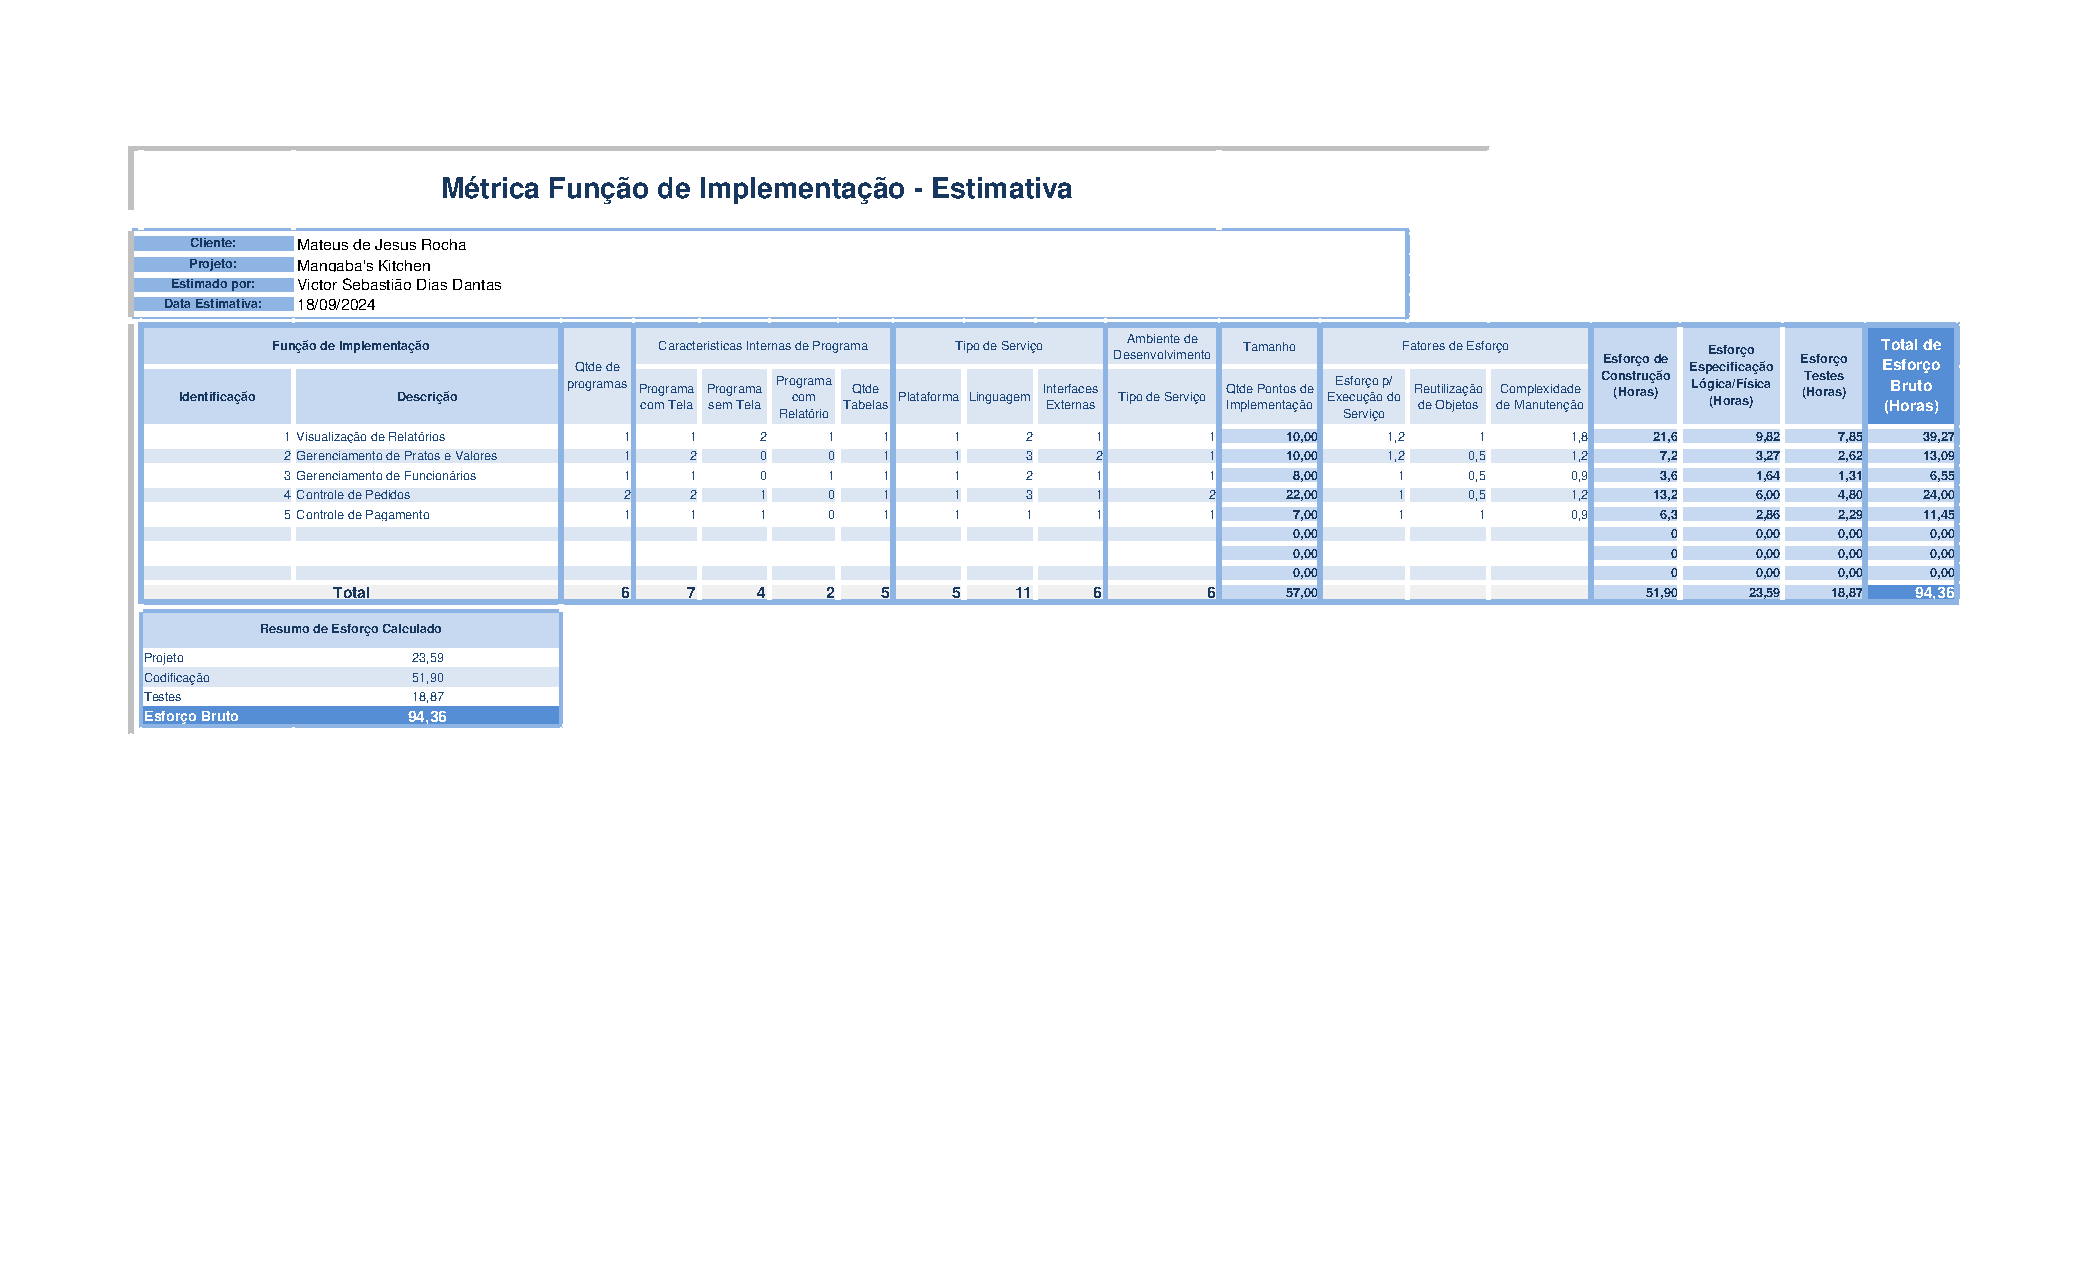
\includepdf[pages=1]{./PDFs/Documento_de_Estimativa.pdf}
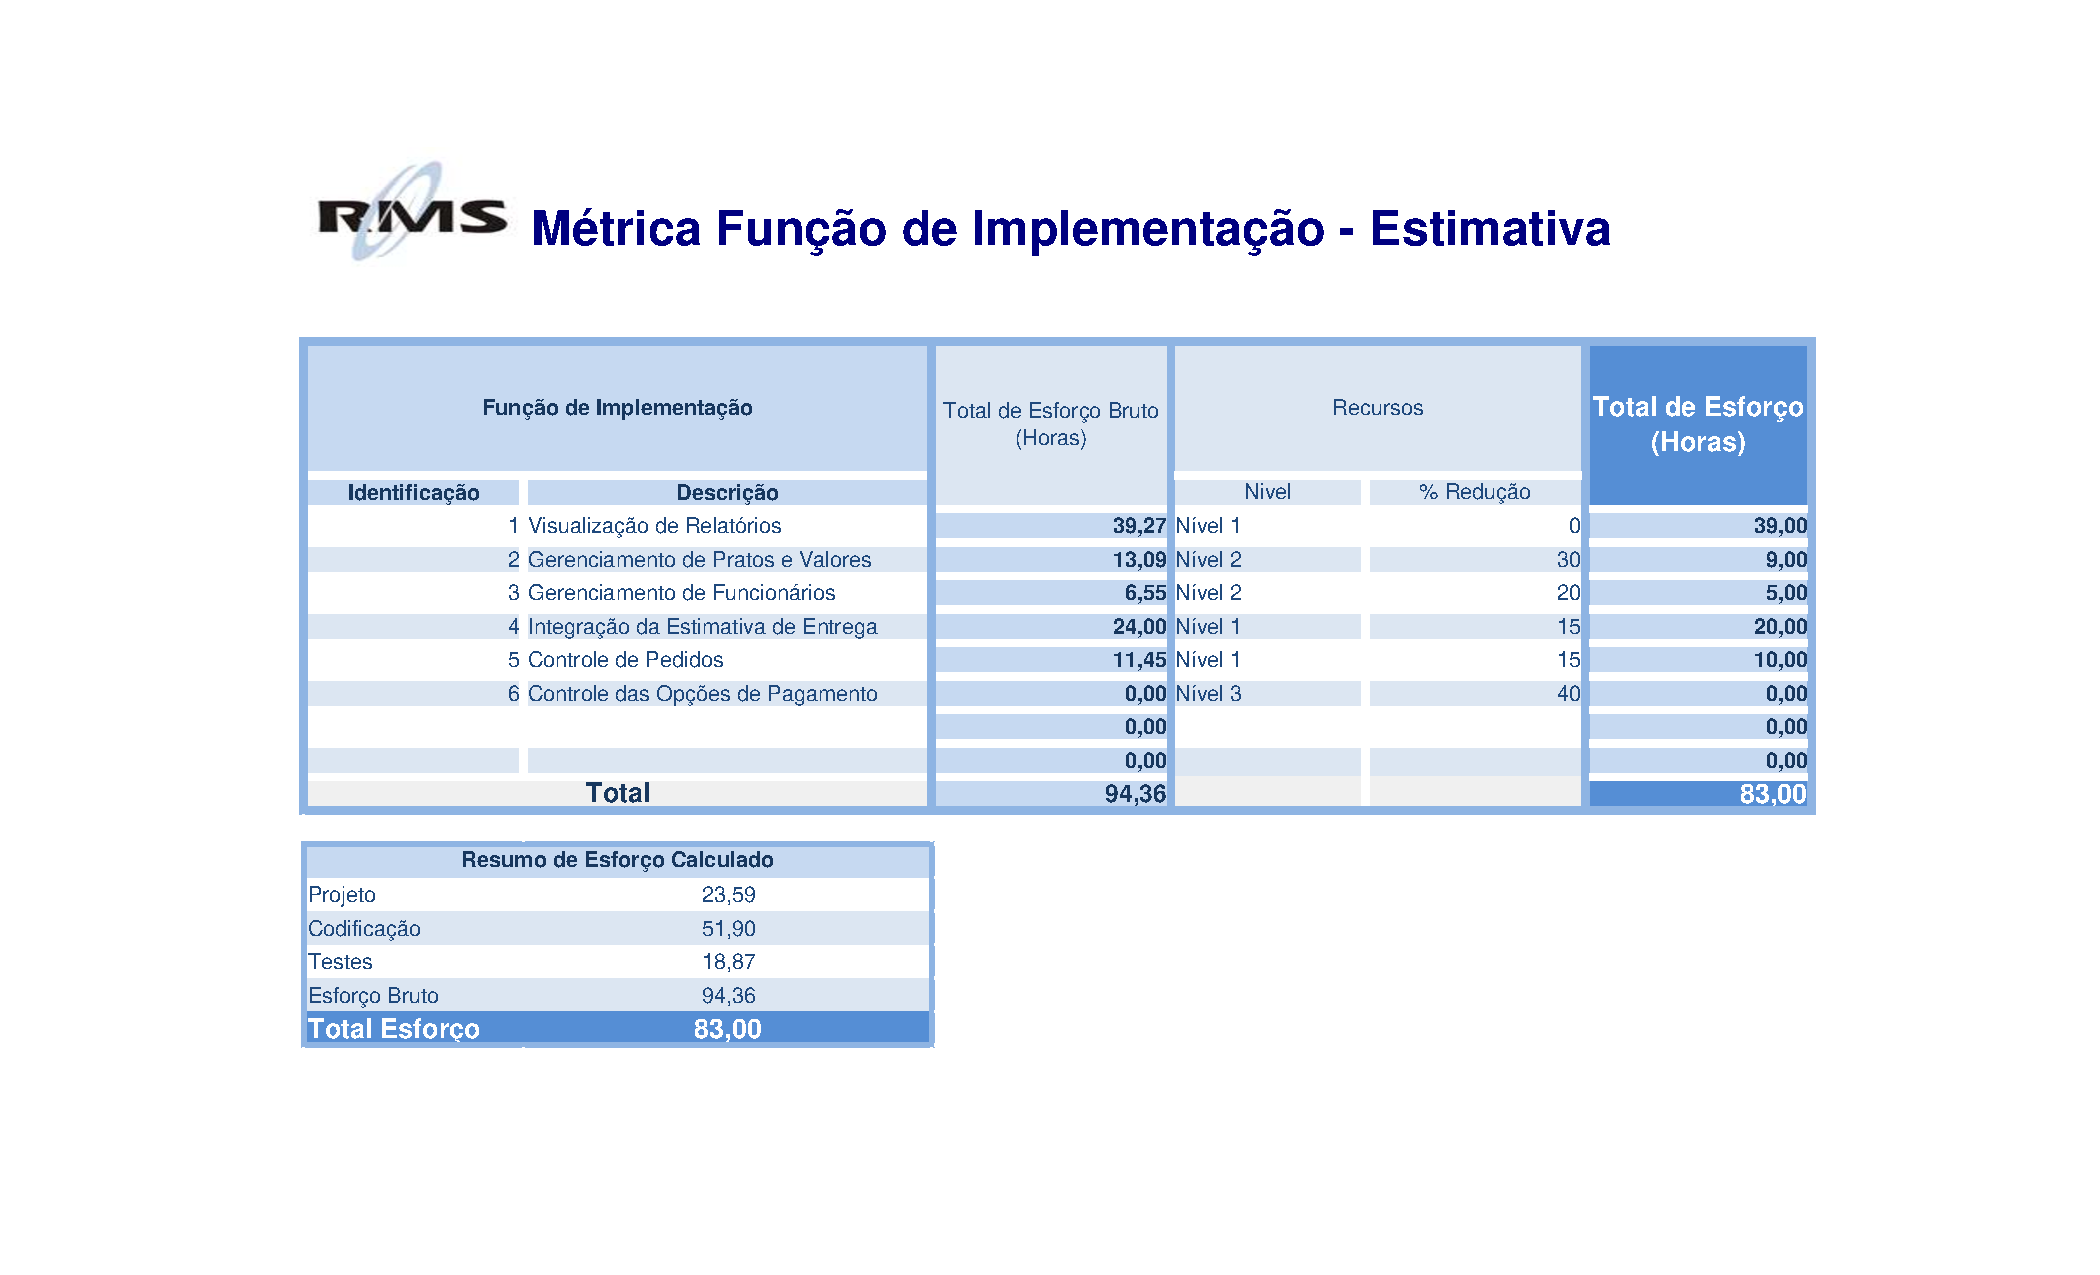
\includepdf[pages=1]{./PDFs/Documento_de_Recursos.pdf}